\chapter{Analisi dei requisiti}
\label{cap:analisi-requisiti}

\intro{Il capitolo è dedicato all'analisi dei requisiti della piattaforma, con l'obiettivo di fornire una visione completa e dettagliata delle funzionalità e delle caratteristiche attese dal sistema. Verranno illustrate le esigenze degli utenti e del contesto operativo, evidenziando le specifiche tecniche e le funzionalità che hanno guidato le scelte progettuali.}\\

%\section{Casi d'uso}

%Per lo studio dei casi di utilizzo del prodotto sono stati creati dei diagrammi.
%I diagrammi dei casi d'uso (in inglese \emph{Use Case Diagram}) sono diagrammi di tipo \gls{uml}\glsfirstoccur dedicati alla descrizione delle funzioni o servizi offerti da un sistema, così come sono percepiti e utilizzati dagli attori che interagiscono col sistema stesso. \\
%Nel contesto del progetto, volto alla creazione di una piattaforma di monitoraggio per applicazioni \emph{web} con strumenti di \gls{apmg} e componenti di intelligenza artificiale per l’analisi automatica dei dati, le interazioni da parte dell’utente sono ridotte allo stretto necessario. Questo approccio minimizza l’intervento manuale, garantendo che le funzionalità principali siano accessibili in maniera intuitiva e diretta. Di conseguenza, i diagrammi dei casi d’uso risultano semplici e in numero limitato, focalizzati sulle operazioni essenziali per la raccolta, l’analisi e la visualizzazione dei dati di monitoraggio.

%\begin{figure}[!h] 
    %\centering 
    %\includegraphics[width=0.9\columnwidth]{usecase/scenario-principale} 
    %\caption{Use Case - UC0: Scenario principale}
%\end{figure}

%\begin{usecase}{0}{Scenario principale}
%\usecaseactors{Sviluppatore applicativi}
%\usecasepre{Lo sviluppatore è entrato nel plug-in di simulazione all'interno dell'IDE}
%\usecasedesc{La finestra di simulazione mette a disposizione i comandi per configurare, registrare o eseguire un test}
%\usecasepost{Il sistema è pronto per permettere una nuova interazione}
%\label{uc:scenario-principale}
%\end{usecase}

\section{Requisiti del sistema}

A seguito di un'attenta attività di analisi del progetto e degli obiettivi tecnici e funzionali prefissati, sono state redatte le tabelle di tracciamento che riassumono in modo strutturato i requisiti individuati. \\
Durante questa fase sono state identificate differenti tipologie di requisiti, distinte sia in base alla loro categoria (funzionale, non funzionale, qualitativo o di vincolo), sia in base alla loro priorità di implementazione (obbligatorio, desiderabile o opzionale).
Per garantire una tracciabilità chiara e univoca, a ciascun requisito è stato assegnato un codice identificativo composto da lettere che ne descrivono la tipologia e l'importanza, secondo la seguente convenzione:
\begin{description}
	\item [R =] Requisito
	\item [F =] Funzionale
    \item [N =] Non funzionale
    \item [Q =] Qualitativo
    \item [V =] Vincolo
    \item [O =] Obbligatorio
    \item [D =] Desiderabile
    \item [Z =] Opzionale
\end{description}

\newpage

Ogni requisito analizzato sarà identificato univocamente dalla seguente notazione:
\begin{center}
    \textbf{R[Priorità][Categoria]-[Numero]}
\end{center}
Dove:

\begin{itemize}
    \item \textbf{Priorità} indica la priorità di implementazione, che può essere O = Obbligatorio, D = Desiderabile, Z = Opzionale;
    \item \textbf{Categoria} la categoria di appartenenza, che può essere F = Funzionale, N = Non funzionale, Q = Qualitativo, V = Vincolo;
    \item \textbf{Numero} un numero progressivo che identifica in modo univoco il requisito all'interno della sua categoria.
\end{itemize}
Nelle tabelle \ref{tab:requisiti-funzionali}, \ref{tab:requisiti-non-funzionali}, \ref{tab:requisiti-qualitativi} e \ref{tab:requisiti-vincolo} sono riportati in modo sintetico tutti i requisiti emersi dall'analisi, classificati in base alla loro priorità e accompagnati da una breve descrizione della relativa funzionalità o vincolo tecnico. \\


\newpage
\subsection{Requisiti funzionali}
I requisiti funzionali descrivono cosa deve fare il sistema.
Sono le funzionalità concrete che la soluzione deve offrire per raggiungere gli obiettivi del progetto.

\begin{table}[h]
\caption{Tabella del tracciamento dei requisiti funzionali}
\label{tab:requisiti-funzionali}
\begin{tabularx}{\textwidth}{lXl}
\hline
\rowcolor[gray]{0.8}
\textbf{Codice} & \textbf{Descrizione} & \textbf{Classificazione}\\
\hline
ROF-1     & Il sistema deve permettere la raccolta automatica di metriche e \emph{log} relativi alla \emph{web application} tramite agenti \emph{OpenTelemetry} o \emph{Elastic APM}. & Obbligatorio \\
\hline

\hline
ROF-2     & Il sistema deve inviare i dati raccolti agli \emph{endpoint} \emph{Elasticsearch} per l'analisi e l'indicizzazione. & Obbligatorio \\
\hline

\hline
ROF-3     & Il sistema deve consentire la creazione di \emph{pipeline} di \emph{log} tramite \emph{Logstash} per filtraggio, trasformazione e inoltro dei dati in \emph{Elasticsearch}. & Obbligatorio \\
\hline

\hline
ROF-4     & Il sistema deve prevedere la configurazione di \emph{Elastic Agents} (\emph{Beats}/\emph{\gls{apm}}) per la raccolta dati della navigazione. & Obbligatorio \\
\hline

\hline
ROF-5     & Il sistema deve generare \emph{dashboard} avanzate e visualizzazioni in \emph{Kibana}, con metriche di \emph{performance}, accesso e flussi utente. & Obbligatorio \\
\hline

\hline
ROF-6     & Il sistema deve permettere la verifica della corretta acquisizione dei dati e la loro indicizzazione in \emph{Elasticsearch}. & Obbligatorio \\
\hline

\hline
ROF-7     & Il sistema deve prevedere lo sviluppo e l'esecuzione di \emph{script} automatizzati in \emph{Python} o \emph{Java} per la simulazione del traffico utente (\emph{Synthetic Monitoring}). & Obbligatorio \\
\hline

\hline
ROF-8     & Deve essere possibile filtrare e ricercare i \emph{log} per \emph{host}, servizio, livello di severità o periodo temporale. & Obbligatorio \\
\hline

\hline
RDF-9     & Il sistema dovrebbe prevedere la configurazione di regole di \emph{alerting} e notifiche in tempo reale per anomalie rilevate. & Desiderabile \\
\hline

\hline
RDF-10     & Il sistema dovrebbe integrare algoritmi di \emph{Machine Learning} per l'individuazione automatica di anomalie. & Desiderabile \\
\hline

\hline
RDF-11     & Il sistema dovrebbe consentire l'esportazione delle \emph{dashboard} o dei risultati delle \emph{query} in formato \gls{pdf}\glsfirstoccur o \gls{csv}\glsfirstoccur. & Desiderabile \\
\hline

\hline
RZF-12     & Il sistema può prevedere un modulo aggiuntivo per la generazione automatica di report periodici delle metriche raccolte. & Opzionale \\
\hline

\hline
RZF-13     & Il sistema può consentire l'importazione automatica delle configurazioni \gls{apm} da ambienti di \emph{test} o \emph{staging}. & Opzionale \\
\hline

\end{tabularx}
\end{table}%

\newpage
\subsection{Requisiti non funzionali}
I requisiti non funzionali definiscono come il sistema deve comportarsi, cioè le sue proprietà di qualità interna.
Non aggiungono nuove funzioni, ma impongono vincoli di prestazioni, sicurezza, disponibilità, scalabilità, affidabilità e manutenibilità.

\begin{table}[h]
\caption{Tabella del tracciamento dei requisiti non funzionali}
\label{tab:requisiti-non-funzionali}
\begin{tabularx}{\textwidth}{lXl}
\hline
\rowcolor[gray]{0.8}
\textbf{Codice} & \textbf{Descrizione} & \textbf{Classificazione}\\
\hline
RON-1    & Il sistema deve essere scalabile e consentire l'aggiunta di nuove fonti di dati o agenti senza compromettere la stabilità. & - Obbligatorio \\
\hline

\hline
RON-2    & Il sistema deve garantire l'affidabilità nella trasmissione e nella conservazione dei dati raccolti. & - Obbligatorio \\
\hline

\hline
RON-3    & La piattaforma deve assicurare un tempo di latenza accettabile nella visualizzazione dei dati (< 5 secondi per l'aggiornamento delle \emph{dashboard}). & - Obbligatorio \\
\hline

\hline
RDN-4    & Il sistema dovrebbe garantire la possibilità di eseguire \emph{test} di carico e stress per valutare la stabilità dell'ambiente. & - Desiderabile \\
\hline

\hline
RDN-5    & Il sistema dovrebbe supportare l'autenticazione per la gestione degli accessi a \emph{Kibana}. & - Desiderabile \\
\hline


\end{tabularx}
\end{table}%


\newpage
\subsection{Requisiti qualitativi}
I requisiti qualitativi specificano le proprietà qualitative che influenzano l'esperienza d'uso e la manutenibilità.
Si concentrano su aspetti percepibili, come semplicità, chiarezza, flessibilità o estendibilità.

\begin{table}[h]
\caption{Tabella del tracciamento dei requisiti qualitativi}
\label{tab:requisiti-qualitativi}
\begin{tabularx}{\textwidth}{lXl}
\hline
\rowcolor[gray]{0.8}
\textbf{Codice} & \textbf{Descrizione} & \textbf{Use Case}\\
\hline
ROQ-1    & L'interfaccia di \emph{Kibana} deve offrire una rappresentazione chiara e intuitiva delle metriche principali. & - Obbligatorio \\
\hline

\hline
ROQ-2    & I dati devono essere visualizzabili in forma aggregata e filtrabile in base a intervalli temporali e categorie di evento. & - Obbligatorio\\
\hline

\hline
ROQ-3    & Le \emph{dashboard} devono presentare una chiara distinzione cromatica tra metriche positive, neutre e anomale. & - Obbligatorio\\
\hline

\hline
RDQ-4    & Le \emph{dashboard} dovrebbero essere personalizzabili dall'utente secondo criteri di interesse (\emph{performance}, accessi, flussi). & - Desiderabile \\
\hline

\hline
RZQ-5    & Il sistema può includere un \emph{layout dark/light mode} o temi grafici personalizzati per una migliore leggibilità. & - Opzionale \\
\hline

\end{tabularx}
\end{table}%

\newpage
\subsection{Requisiti di vincolo}
Impongono limitazioni o condizioni esterne al progetto: ambienti, tecnologie, compatibilità, strumenti, standard aziendali o legali.

\begin{table}[H]
\caption{Tabella del tracciamento dei requisiti di vincolo}
\label{tab:requisiti-vincolo}
\begin{tabularx}{\textwidth}{lXl}
\hline
\rowcolor[gray]{0.8}
\textbf{Codice} & \textbf{Descrizione} & \textbf{Use Case}\\
\hline
ROV-1    & Il sistema deve utilizzare i prodotti della suite \emph{Elastic Stack} (\emph{Elasticsearch, Logstash, Kibana, Beats, APM Server/Agent}). & - Obbligatorio \\
\hline

\hline
ROV-2    & L'ambiente operativo deve essere \emph{Linux} (\emph{Red Hat} o distribuzioni equivalenti). & - Obbligatorio \\
\hline

\hline
ROV-3    & Tutti i componenti \emph{software} devono essere compatibili con la versione di \emph{Linux} installata sull'ambiente aziendale (es. \emph{Ubuntu 22.04 LTS} o \emph{Red Hat 9}). & - Obbligatorio \\
\hline

\hline
ROV-4    & Le componenti devono rispettare le seguenti versioni minime:

\begin{itemize}
    \item \emph{Python} >= 3.10
    \item \emph{Java} >= 16
    \item \emph{Node.js} >= 17
    \item \emph{Logstash} >= 8.10
    \item \emph{Kibana} >= 8.10
    \item \emph{Beats} >= 8.10
    \item \emph{APM Server} >= 8.10
    \item \emph{Elasticsearch} >= 8.10
    \item \emph{OpenTelemetry} >= 1.0
\end{itemize}& - Obbligatorio \\
\hline

\hline
ROV-5    & La \emph{web application} deve essere compatibile con i principali \emph{browser} (\emph{Chrome} >= 120, \emph{Firefox} >= 115, \emph{Edge} >= 120, \emph{Apple Safari} >= 15). & - Obbligatorio \\
\hline

\hline
ROV-6    & Tutte le configurazioni devono essere eseguite in un ambiente \emph{Docker} o su infrastruttura fornita da Kirey Group. & - Obbligatorio \\
\hline

\hline
RDV-7    & La documentazione tecnica deve essere redatta in formato \emph{Markdown}, \emph{LaTeX} o \gls{pdf}, seguendo gli standard aziendali. & - Desiderabile \\
\hline

\hline
RDV-8    & Il sistema dovrebbe consentire la distribuzione automatizzata tramite \emph{Docker Compose}. & - Desiderabile \\
\hline

\end{tabularx}
\end{table}

\newpage
\section{Riepilogo dei requisiti}

\begin{center}
\captionof{table}{Riepilogo dei requisiti}
\label{tab:requisiti-riepilogo}
\begin{tabular}{|l|c|c|c|c|}
\hline
\rowcolor[gray]{0.8}
\textbf{Tipologia} & \textbf{Obbligatorio} & \textbf{Desiderabile} & \textbf{Opzionale} & \textbf{Totale} \\
\hline
\textbf{Funzionali} & 8 & 3 & 2 & 13 \\
\hline

\hline
\textbf{Non funzionali} & 3 & 2 & 0 & 5 \\
\hline

\hline
\textbf{Qualitativi} & 3 & 1 & 1 & 5 \\
\hline

\hline
\textbf{Di Vincolo} & 6 & 2 & 0 & 8 \\
\hline

\hline
\textbf{Totale} &  &  &  & 31 \\
\hline

\end{tabular}
\end{center}

\newpage
\section{Rappresentazione architetturale preliminare}
La rappresentazione architetturale descrive la struttura della soluzione proposta, evidenziando le principali componenti coinvolte nel sistema di \gls{apm} e le loro relazioni. \\
Essa costituisce il collegamento tra la fase di analisi dei requisiti e la successiva implementazione pratica. I dettagli tecnici e i diagrammi della soluzione verranno approfonditi nel capitolo dedicato alla progettazione architetturale.


\subsection{Struttura generale della soluzione di monitoraggio}
La soluzione di \gls{apm} proposta si fonda su un'architettura modulare che integra i principali componenti dell'\emph{Elastic Stack}, garantendo un sistema di osservabilità completo.  
L'applicazione \emph{Spring PetClinic} viene monitorata attraverso due agenti: l'\emph{APM Agent Java}, che raccoglie metriche e tracce lato \emph{backend}, e il \emph{RUM Agent JavaScript}, che monitora le prestazioni e le interazioni utente sul \emph{frontend}.  
I dati generati dagli agenti vengono inviati al \emph{Fleet Server}, che gestisce in modo centralizzato gli \emph{Elastic Agent} e i relativi moduli, tra cui l'\emph{APM Server}.  
Quest'ultimo riceve, elabora e normalizza i dati di monitoraggio, inoltrandoli successivamente a \emph{Elasticsearch} per l'indicizzazione e la conservazione.  
Le informazioni archiviate vengono poi esplorate e analizzate tramite \emph{Kibana}, che offre funzionalità avanzate di visualizzazione, creazione di \emph{dashboard} interattive e configurazione di regole di \emph{alerting} e \emph{Synthetic Monitoring}.  


\subsection{Integrazione dei componenti principali}
L'architettura della soluzione di monitoraggio si compone dei seguenti moduli principali:
\begin{itemize}
    \item \textbf{Elasticsearch:} motore di ricerca e analisi distribuito che gestisce la memorizzazione, l'indicizzazione e l'interrogazione dei dati provenienti dagli agenti di monitoraggio in tempo reale;
    
    \item \textbf{Kibana:} interfaccia di visualizzazione e analisi integrata con \emph{Elasticsearch}, consente di visualizzare metriche e tracce applicative, creare \emph{dashboard} personalizzate e configurare regole di \emph{alerting} per il monitoraggio del sistema;
    
    \item \textbf{Fleet:} componente centralizzato per la gestione e la configurazione degli agenti \emph{Elastic}. Attraverso il \emph{Fleet Server}, coordina la comunicazione con gli \emph{Elastic Agents};
    
    \item \textbf{Logstash:} sistema di \emph{data processing} che consente di raccogliere, trasformare e inoltrare i dati di log e metriche da diverse fonti verso \emph{Elasticsearch};

    \item \textbf{Elastic Agent:} agente unificato che integra funzionalità di raccolta dati, sicurezza e monitoraggio. Gestito tramite \emph{Fleet}, può essere configurato per includere moduli specifici come \emph{APM Server} e \emph{Beats} per la raccolta di metriche di sistema e log;

    \item \textbf{APM Server:} incluso all'interno dell'\emph{Elastic Agent}, riceve i dati di telemetria provenienti dagli agenti applicativi (\gls{apmg} e \gls{rumg}\glsfirstoccur), li elabora e li inoltra a \emph{Elasticsearch} in formato ottimizzato per la successiva analisi e visualizzazione;

    \item \textbf{APM Agent Java:} agente integrato nel \emph{backend} dell'applicazione \emph{Spring PetClinic}, responsabile del tracciamento automatico delle transazioni, delle chiamate ai servizi e delle operazioni sul database;
    
    \item \textbf{RUM Agent JavaScript:} agente di monitoraggio \gls{rumg} eseguito nel \emph{frontend} dell'applicazione, che raccoglie dati sulle interazioni utente, sui tempi di caricamento delle pagine e sulle prestazioni percepite nel browser;
    
\end{itemize}


\begin{figure}[!h] 
    \centering 
    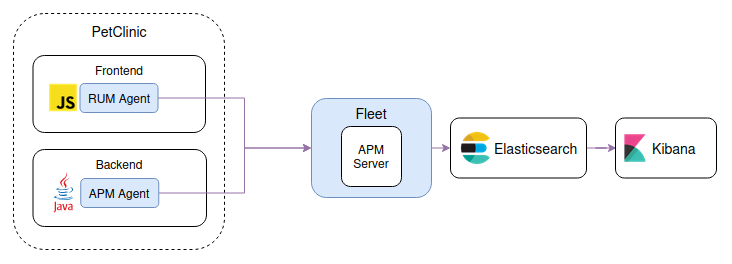
\includegraphics[width=\columnwidth]{Integrazione_APM.png} 
    \caption{Figura 3.1 - Integrazione tra componenti}
\end{figure}


\subsection{Applicazione di riferimento: Spring PetClinic}
Per la sperimentazione del sistema di \gls{apm} è stata utilizzata come applicazione di riferimento \emph{Spring PetClinic}, una \emph{web application} \emph{open source} sviluppata in \emph{Java} e basata sul \emph{framework} \emph{Spring Boot}.  
La scelta di \emph{PetClinic} è motivata dalla sua architettura chiara e ben documentata, composta da un livello di presentazione (\emph{controller} e \emph{template}), un livello logico (servizi) e un livello di persistenza (\emph{repository} e \emph{database} \gls{mysqlg}\glsfirstoccur).  
Tale struttura consente di osservare comportamenti applicativi realistici, come chiamate \gls{httpg}\glsfirstoccur, interazioni con il \emph{database} e logiche di \emph{business}, fornendo un contesto ideale per testare le funzionalità di monitoraggio offerte da \emph{Elastic APM} e \emph{OpenTelemetry}.  

\begin{figure}[!h] 
    \centering 
    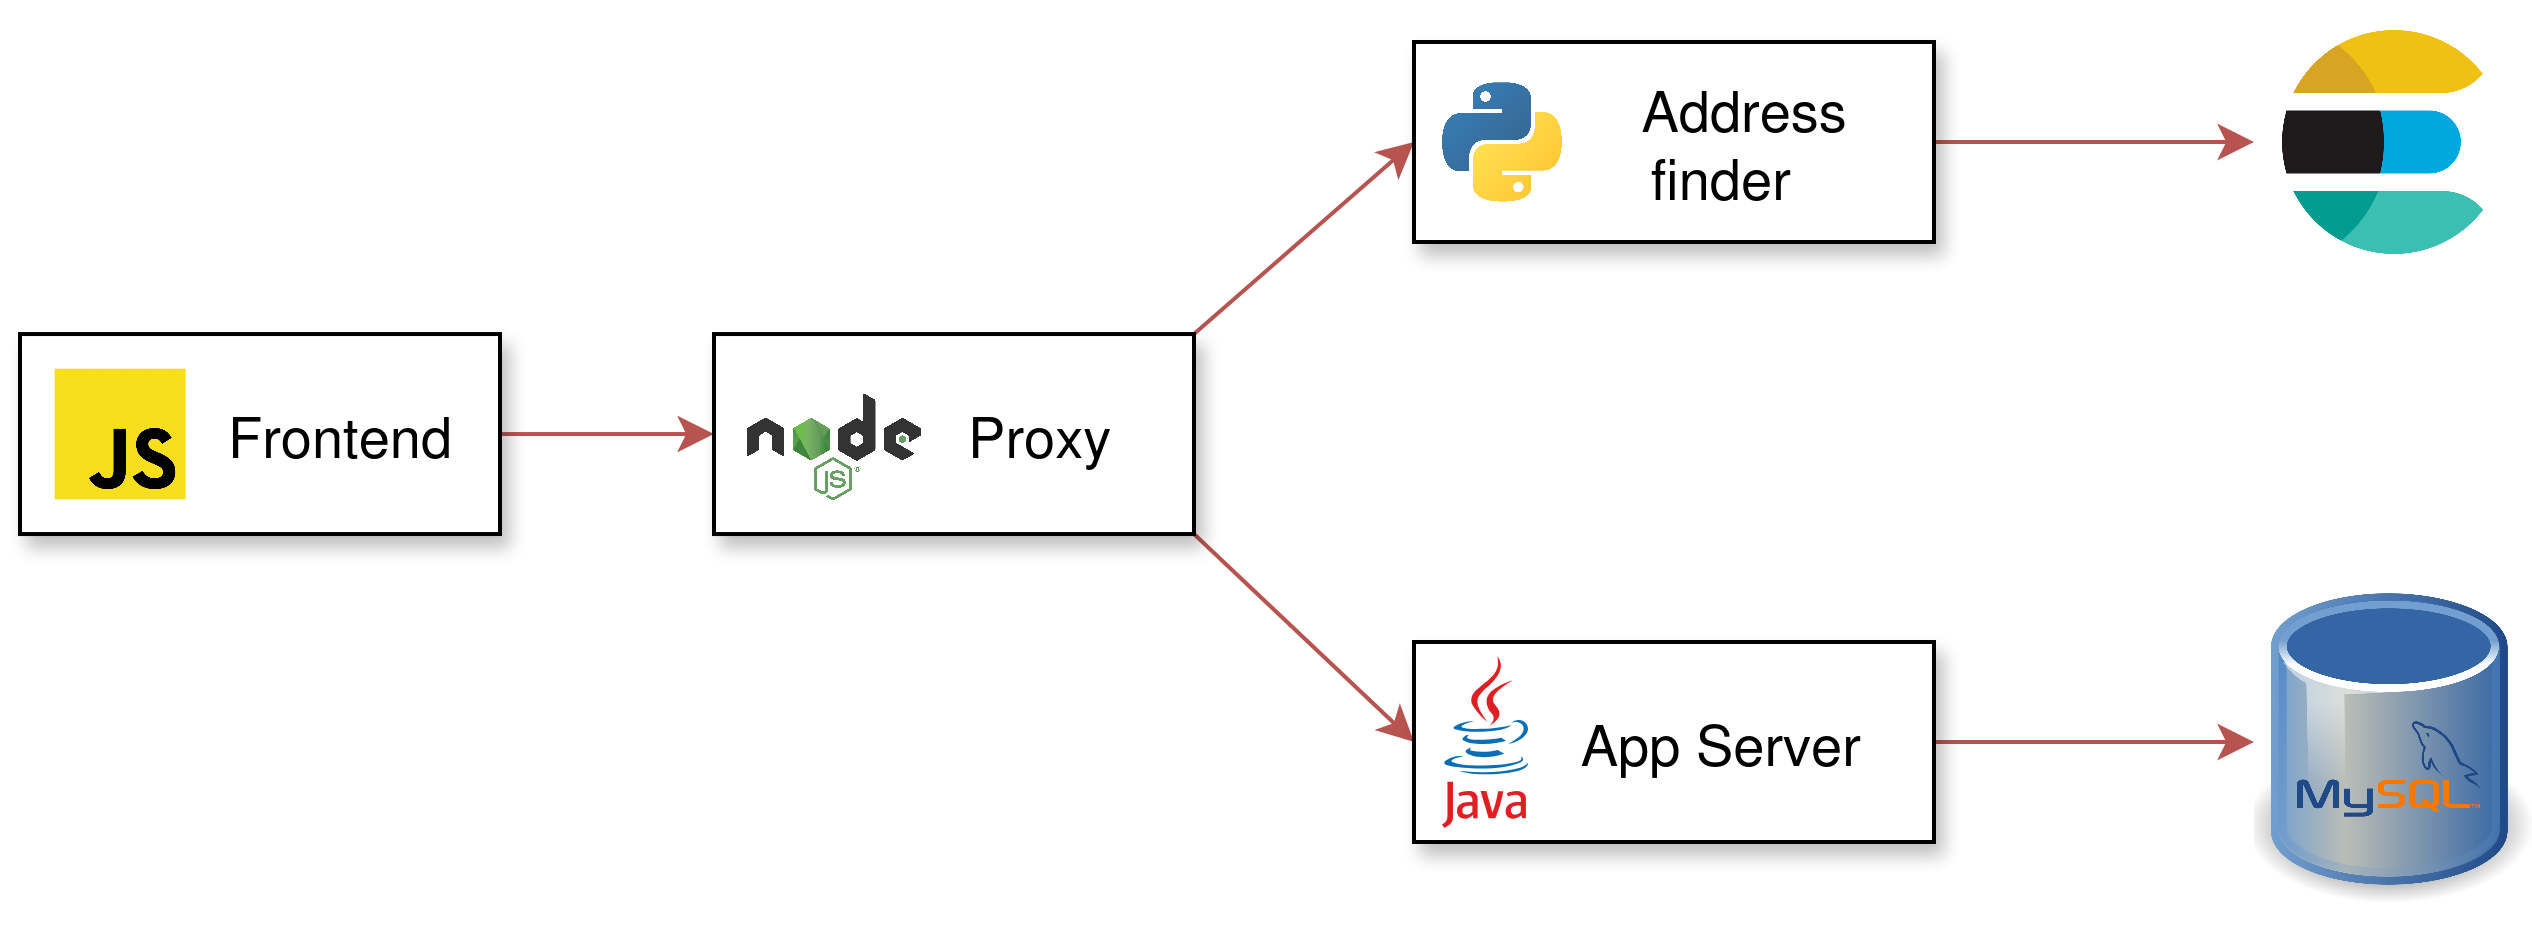
\includegraphics[width=\columnwidth]{Architettura_PetClinic.png} 
    \caption{Figura 3.2 - Architettura di Spring PetClinic}
\end{figure}


L'applicazione \emph{PetClinic} verrà quindi utilizzata come caso di studio per la validazione della soluzione di monitoraggio proposta, analizzando successivamente il modo in cui i diversi moduli architetturali interagiscono con essa.
\newpage

\subsection{User Stories e scenari di utilizzo}
Le seguenti \emph{user stories} descrivono brevemente i principali scenari di utilizzo del sistema di \gls{apm}, evidenziando gli obiettivi e le esigenze degli utenti tecnici aziendali che operano sulla piattaforma di monitoraggio.  
L'unico attore considerato è l'\emph{Observability Engineer}, figura responsabile della configurazione, analisi e manutenzione del sistema all'interno dell'azienda.


\begin{longtable}{|p{1cm}|p{8cm}|p{3cm}|}
\caption{User Stories}
\label{tab:user-stories} \\
\hline
\rowcolor[gray]{0.8}
\textbf{ID} & \textbf{User Story} & \textbf{Obiettivo} \\
\hline
\endfirsthead

\hline
\textbf{US1} & Come \emph{Observability Engineer}, voglio analizzare i tempi medi di risposta degli \emph{endpoint} dell'applicazione per individuare colli di bottiglia o degradi di \emph{performance}. & Ottimizzare le prestazioni applicative. \\
\hline

\textbf{US2} & Come \emph{Observability Engineer}, voglio monitorare l'utilizzo di \gls{cpug}, memoria e connessioni per valutare la stabilità del sistema. & Garantire la corretta gestione delle risorse. \\
\hline

\textbf{US3} & Come \emph{Observability Engineer}, voglio rilevare e classificare errori e anomalie dai \emph{log} per identificare rapidamente le cause dei malfunzionamenti. & Migliorare l'affidabilità del sistema. \\
\hline

\textbf{US4} & Come \emph{Observability Engineer}, voglio configurare regole di \emph{alerting} in \emph{Kibana} per essere notificato in caso di anomalie. & Ridurre i tempi di risposta agli incidenti. \\
\hline

\textbf{US5} & Come \emph{Observability Engineer}, voglio visualizzare le metriche aggregate in \emph{dashboard} personalizzate. & Facilitare l'analisi e la comunicazione dei risultati. \\
\hline

\textbf{US6} & Come \emph{Observability Engineer}, voglio visualizzare in \emph{Kibana} le metriche di prestazione del \emph{backend} (tempi medi di risposta, \emph{throughput}, tasso di errore, durata media delle transazioni) per valutare lo stato di salute dell'applicazione. & Monitorare le prestazioni e la stabilità del servizio. \\
\hline

\textbf{US7} & Come \emph{Observability Engineer}, voglio visualizzare metriche di utilizzo delle risorse di sistema (\gls{cpug}, memoria, disco, rete) per individuare potenziali colli di bottiglia. & Ottimizzare l'efficienza del sistema. \\
\hline

\textbf{US8} & Come \emph{Observability Engineer}, voglio analizzare in \emph{Kibana} le metriche relative al comportamento degli utenti (\emph{page load time}, errori JavaScript, interazioni lente) raccolte dal \emph{RUM Agent}. & Migliorare l'esperienza utente. \\
\hline

\textbf{US9} & Come \emph{Observability Engineer}, voglio correlare in un'unica \emph{dashboard} le metriche di infrastruttura, \emph{application performance} e \emph{user experience}, per ottenere una visione completa del sistema. & Favorire un'analisi integrata e diretta delle anomalie. \\
\hline

\textbf{US10} & Come \emph{Observability Engineer}, voglio integrare l'\emph{APM Agent Java} e il \emph{RUM Agent JavaScript} per raccogliere rispettivamente metriche di \emph{backend} e \emph{frontend}. & Avere una visione completa del comportamento dell'applicazione. \\
\hline

\textbf{US11} & Come \emph{Observability Engineer}, voglio configurare e gestire gli agenti tramite \emph{Fleet} per garantire una distribuzione e un aggiornamento centralizzati. & Semplificare la manutenzione e ridurre gli errori di configurazione. \\
\hline

\textbf{US12} & Come \emph{Observability Engineer}, voglio eseguire \emph{test} sintetici periodici per monitorare la disponibilità e i tempi di risposta delle pagine. & Garantire la continuità operativa. \\
\hline

\textbf{US13} & Come \emph{Observability Engineer}, voglio esportare le \emph{dashboard} in formato \gls{pdf} o \gls{csv} per la condivisione all'interno del team. & Documentare e condividere le analisi in modo efficace. \\
\hline

\textbf{US14} & Come \emph{Observability Engineer}, voglio ricevere notifiche automatiche via email quando vengono superate determinate soglie di prestazione. & Automatizzare la gestione degli incidenti e migliorare il tempo di reazione. \\
\hline

\textbf{US15} & Come \emph{Observability Engineer}, voglio configurare in \emph{Kibana} job di \emph{Machine Learning} per l’individuazione automatica di anomalie. & Rilevare comportamenti anomali senza intervento manuale. \\
\hline

\textbf{US16} & Come \emph{Observability Engineer}, voglio visualizzare in \emph{Kibana} i risultati dei job di \emph{Machine Learning} (anomalie, trend, previsioni) integrati nelle \emph{dashboard} operative. & Integrare l'analisi automatica con la visualizzazione interattiva dei dati. \\
\hline

\end{longtable}


%\section{Conclusioni}
%Il presente capitolo ha illustrato l'analisi dei requisiti del sistema di \gls{apm}, la loro classificazione e la relativa mappatura sulle componenti principali dell'architettura prevista.  
